\chapter{State of the Art} \label{ch:state-of-the-art}

\section{Problem 1 - Tactile Perception} \label{sec:lit-rev-problem-1}

Based on the contact model categories described above, the most representative is \gls{sf} since these models can provide descriptions of the contact surface topology, and thus enable the solving of the \gls{iep} by deriving surface features for pose estimation. Furthermore in order to manipulate objects in-hand and ensuring force closure the friction Representation is needed. An illustration of the system as a \gls{sf} can be seen in ..., while . 

% \begin{center}
%     \renewcommand{\arraystretch}{1.2}
%     \begin{minipage}{.48\linewidth}
%         \vspace{0pt}
%         \centering
%         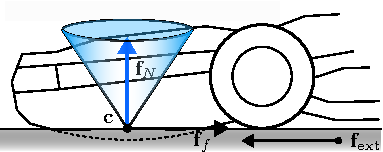
\includegraphics[width=.95\textwidth]{chapters/modeling/fig/friction-cone-schematic.pdf}
%     \end{minipage}%
%     \hfill%
%     \begin{minipage}{.48\linewidth}
%         \vspace{0pt}
%         \centering
%         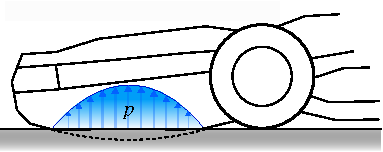
\includegraphics[width=.95\textwidth]{chapters/modeling/fig/contact-surface.pdf}
%     \end{minipage}%
%     %    
%     \vspace{15pt}
%     %
%     \begin{minipage}[t]{.48\linewidth}
%         \vspace{0pt}
%         \captionsetup{type=figure}
%         \captionof{figure}{Single point contact model between compliant manipulator surface and object surface.}
%         \label{fig:contact-single-point}
%     \end{minipage}%
%     \hfill%
%     \begin{minipage}[t]{.48\linewidth}
%         \vspace{0pt}
%         \captionsetup{type=figure}
%         \captionof{figure}{Contact model of the pressure distribution $p(r)$ caused by the increased force applied from the \gls{ee}'s finger to the object.}
%         \label{fig:contact-surface}
%     \end{minipage}%
% \end{center}


% subcategories of sf models
Within the category of \gls{sf} models a method fit for this project's use case is to be chosen to solve problem \ref{prob:1}. \gls{sf} models can furthermore be divided up into three different categories: \gls{aebm}, \gls{efm} and \gls{fem} \cite{a-modified-elastic-foundation-contact-model-for-application-in-3d-models-of-the-prosthetic-knee}. \medskip

% reformulate
\gls{aebm} are theoretical formulations of elastic contact areas and the stresses on both the surfaces and the sub-surfaces of the contacting bodies. These types of formulations however are often restricted to describing simple contact geometries. The first of such models was introduced by Heinrich Rudolf Hertz in 1882\cite*{on-the-contact-of-rigid-elastic-solids-and-on-hardness} and is still used for simple contact cases. In the formulation of the Hertzian contact model two assumptions are made: Objects in contact are made of linear elastic materials and only small contact deformations occur compared to the dimension of object. However, robotic \gls{ee} fingertips are often made of nonlinear elastic materials and for that reason the Hertzian contact model does not represent the type of contact in this project\cite[Chapter 37]{handbook-of-robotics}. To improve on the Hertzian model, a more generic formulation can be made which extends the model from linear to nonlinear elastic contacts\cite*{modeling-of-contact-mechanics-and-friction-limit-surfaces-for-soft-fingers-in-robotics-with-experimental-results}\cite*{the-haptic-and-perceptional-characteristics-of-an-anthropomorphic-curved-soft-finger-structure}. This power-law formulation subsumes the Hertzian contact theory while assuming a circular contact area. Other models have been purposed which combine the descriptions of both friction-contact and the shear-torsion as experienced by the bodies\cite{the-sliding-of-robot-fingers-under-combined-torsion-and-shear-loading}. However, in order to more accurately describe the contacts involving robot fingers, viscoelastic soft contact model appear more relevant due to such fingers often being made of materials which show viscoelastic properties e.g., rubber, silicone and polymers. Simple models such as  Kelvin-Voigt's\cite*{viscoelasticity} and Maxwell's\cite{on-the-dynamical-theory-of-gases} models describe the interaction between strain and stress as a spring damper system in a serial or in a parallel configuration respectively. Models which expand on this idea describe the reacting force as the product of the temporal and the elastic response, while incorporating previous stress responses\cite{mechanical-properties-and-active-remodeling-of-blood-vessels}.
To simplify this formulation alternatives have been developed to assume no past stress \cite{modeling-of-viscoelastic-contacts-and-evolution-of-limit-surface-for-robotic-contact-interface}\cite*{characteristics-of-contact-and-limit-surface-for-viscoelastic-fingers}\cite*{effect-of-layer-compliance-on-frictional-behavior-of-soft-robotic-fingers}.

Upon these, more modern techniques have been developed which has seen use in similar use cases as the ones of interest in this project.

% modern methods....
% AEBM modern method 1 - red sheat polygon - reformulate
Friction constraints are derived based on general expressions for non-planar contacts of elastic bodies, taking into account the local geometry and structure of the objects in contact. These constraints are then formulated as a linear complementarity problem, the solution of which provides the normal and frictional forces applied at each contact, as well as the relative velocity of the bodies involved. This approach captures frictional effects such as coupling between tangential force and frictional torque. We illustrate this method by analyzing manipulation tasks performed by an anthropomorphic robotic hand equipped with soft fingerpads\cite*{soft-finger-model-with-adaptive-contact-geometry-for-grasping-and-manipulation-tasks}.
% AEBM modern method 2 - A new algorithm for computing the indentation of a rigid body - reformulate
In this paper the contact problem between a rigid indenter of arbitrary shape and a viscoelastic half-
space is considered. Under the action of a normal force the penetration of the indenter and the
distribution of contact pressure change. We wish to find the relations which link the pressure
distribution, the resultant force on the indenter and the penetration on the assumption that the surfaces
are frictionless\cite*{a-new-algorithm-for-computing-the-indentation-of-a-rigid-body-of-arbitrary-shape-on-a-viscoelastic-half-space}
% AEBM modern method 3 - Love's Formulation
Tactile sensing is a key enabling technology to develop complex behaviors for robots
interacting with humans or the environment. This paper discusses computational aspects playing
a significant role when extracting information about contact events\cite*{contact-modelling-and-tactile-data-processing-for-robot-skins}.



% a useful overview
% 

% Boussinesq–Cerruti’s

% Love's formulation 

\gls{efm} are 

% paper: (2007) A modified elastic foundation contact model for application in 3D models of the prosthetic knee






% Analytical models are the easiest to calculate but are restricted to simple geometries
% FEMs have been increasingly used over recent years given that they supply information about the sub-surface stresses and strain in volumetric finite elements. However, they are excessively time consuming for fast simulation in dynamic grasping and manipulation models
% EFMs were developed in order to allow a simple discrete contact calculation in more general surface geometries, modelling the deformable part of the contact as a layer over a rigid base, and a series of discrete and independent springs in the contact normal


% 1) I want to model contacts
% 2) there exist 8 different modeling taxonolies
% 3) three are most common
% 	3.a) explain each of the three 
% 4) since soft supports the behavior we want we choose that one
% 5) what method categories exist within soft finger modelling




\section{Problem 2 - Pose Estimation} \label{sec:lit-rev-problem-2}

\section{Problem 3 - In-Hand Manipulation} \label{sec:lit-rev-problem-3}